\chapter{Appendix}
\section{Climate Engineering and CDR options}\label{sec:app_ce}
Geo-engineering is defined as the deliberate large-scale intervention in the Earth's climate system to moderate global warming \citep{shepherd2009}. Geo-engineering methods can be divided into two categories: Carbon dioxide removal (CDR) techniques which sequester atmospheric \ce{CO_2} or prevent release of \ce{CO_2}, and solar radiation management (SRM) techniques that reflect a small percentage of the Sun's radiation back into space, causing the Earth to absorb less solar radiation, and eventually cool. \Cref{fig:app_geo} illustrates possible technologies and the region of application (land, ocean, atmosphere). Enhanced weathering is not explicity mentioned but comes under \textit{Alkalinity Addition}. 
\begin{figure}[h]
\centering
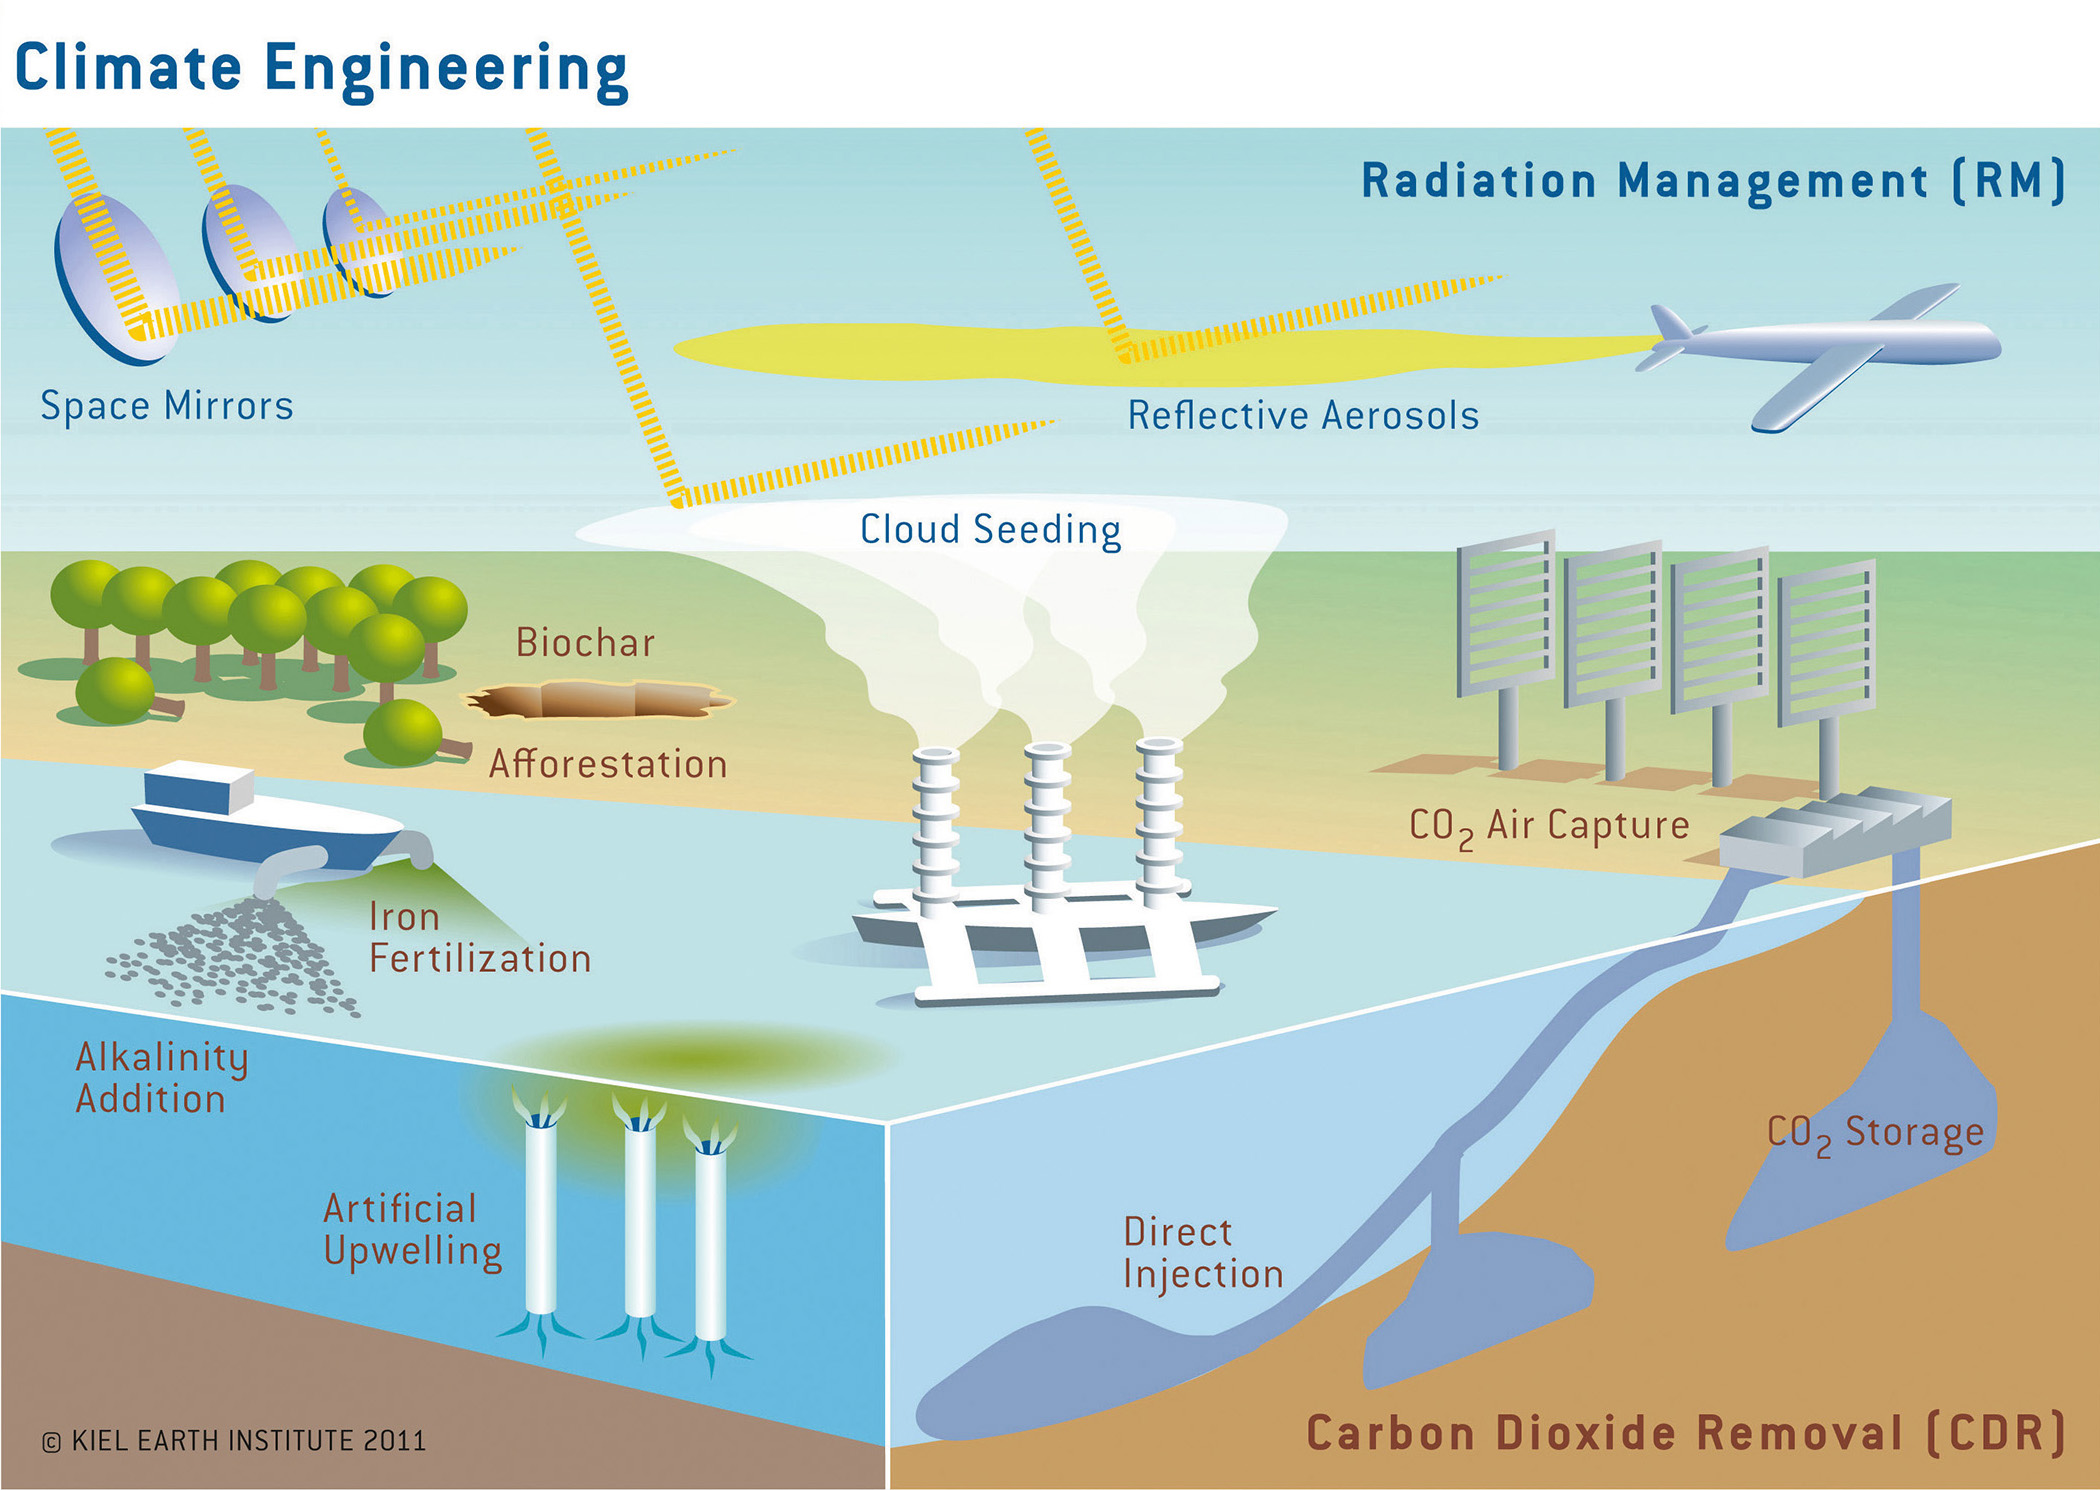
\includegraphics[scale=0.4]{climate_engineering.jpg}
\caption{Schematic illustration of CE technologies. Source: kiel-earth-institute - own work, https://commons.wikimedia.org/w/index.php?curid=38682676}
\label{fig:app_geo}
\end{figure}

\section{Enhanced Weathering and Mineral Carbonation}
Mineral carbonation is another method of carbon sequestration and involves the reaction of a near-pure stream of \ce{CO_2} (coming from the capture-stage of a power plant) with metal oxide bearing minerals to form insoluble carbonates. This process can be \textit{in-situ} where \ce{CO_2} is pumped into geologic sites containing silicate rocks or \textit{ex-situ} where rocks are mined, crushed, and then reacted with a \ce{CO_2} stream at high- temperature and pressure \citep{coninck2005ipcc}. An example of general carbonation reaction is shown in \cref{eq:mincarbonation}, \ce{CO_2} reacts with  metal oxides (indicated here as MO, where M is a divalent metal, e.g., calcium, magnesium, or iron) to form the corresponding metal carbonate and give heat.
\begin{equation}\label{eq:mincarbonation}
\ce{MO + CO_{2} -> MCO_{3} + heat}
\end{equation}
The differences between mineral carbonation and enhanced weathering are shown in \Cref{tab:app_comparison}.
\begin{table}[h]
        \centering
        \def\arraystretch{1.5}
        %caption{Solution with \texttt{tabularx}}
\begin{tabularx}{\textwidth}{ |X|X|X|X| }
  \hline
   & \textbf{Enhanced Weathering} & \textbf{Mineral Carbonation} \\
  \hline 
   \textbf{Conditions}  &  \ce{CO_2} dissolved in water reacts with mineral at ambient temperature and pressure & \ce{CO_2} gas-stream reacts with  minerals at elevated temperature, pressure or both  \\
   \hline 
   \textbf{\ce{CO_2} source} & Atmosphere & Near-pure \ce{CO_2} stream from capture-stage of power plants/industries \\ 
   \hline
   \textbf{Reaction products} & Dissolved metal cations, silica, trace carbonates & Metal carbonates and silica \\ 
  \hline
 \end{tabularx}
 \label{tab:app_comparison}
 \caption{Summary of main differences between Enhanced weathering and Mineral carbonation}
\end{table}
\section{Molecular formula of olivine}\label{sec:mol_app}
\begin{equation*}
\begin{aligned}
&\text{wt.\ $\%$ of Fe in \ce{Fe2O3}} = \textfrac{Molecular Wt. of Fe}{Molecular Wt. of \ce{Fe2O3}} = \textfrac{56}{120}\\[0.5cm]
&\si{\mole\percent} \text{of Fe} = \textfrac{wt. $\%$ of Fe in \ce{Fe2O3} $\times$ wt.\ $\%$ of \ce{Fe2O3}}{molecular mass of Fe}=\left(\textfrac{56}{120}\right)\left(\textfrac{\SI{6.75}{\percent}}{56}\right)=\num{0.05625}\\[0.5cm]
&\text{wt.\ $\% $ of Mg in MgO} = \textfrac{Molecular Wt. of Mg}{Molecular Wt. of MgO} =  \textfrac{24.3}{40.3}
\end{aligned}
\phantom{\hspace{0cm}}
\end{equation*}
\begin{equation*}
\begin{aligned}
&\si{\mole\percent}\ \text{of Mg in sample} = \textfrac{wt.\ $\%$ of Mg in MgO $\times$ wt.\ $\%$ of MgO}{molecular mass of Mg}=\textfrac{24.3 $\times$ 44.99}{40.3 $\times$ 24.3}=\num{0.8957}\\[0.5cm]
&\text{Molar ratio} = \textfrac{Mg}{Fe}=\textfrac{0.8957}{0.05625}=\num{15.92}\\[0.5cm]
&\textfrac{x}{1-x} =\num{16.92}\\[0.5cm]
&\text{x} =\num{0.941}\\[0.5cm]
&\text{Therefore, the chemical formula is \ce{Mg_{1.88}Fe_{0.12}SiO_4}}
\end{aligned}
\phantom{\hspace{0cm}}
\end{equation*}

\section{BET analyses}\label{sec:BET_a}
The specific surface area (SSA) of a mineral surface is found using a method developed by Brunauer–Emmett–Teller (BET) \citep{brunauer1938}. It involves the adsorption of an inert gas, such as nitrogen, to the mineral surface at low temperature; forming a mono-layer thick film. The change in \ce{N2} pressure is measured and the corresponding gas adsorbed is calculated \citep{brantley2000,rimstidt2013}. The total surface area (TSA), also called BET surface area\; \cite{Brantley2008b}, is calculated by multiplying the specific surface area with the sample weight. 

Two surface area analyses were performed for each of the two grain types, i.e., \SI{<63}{\micro\meter} and \SIrange[range-units = single,range-phrase = --]{0}{3}{\milli\metre}. No chemical pre-treatment was done on the samples, but they were heated in near-vacuum conditions at a rate of \SI{5}{\degreeCelsius\per\minute} to \SI{300}{\degreeCelsius} and held at that temperature for \SI{120}{\minute} to remove adsorbed water. For each analysis, \SIrange[range-units = single,range-phrase = --]{5}{6}{\gram} of the sample was taken in a long-necked tube, cleaned with acetone and dried overnight in an oven at \SI{50}{\degreeCelsius}, with a stem diameter of \SI{12}{\milli\meter} and a rounded bulb at the bottom. The inclusion of bigger grain particles (\SI{>2}{mm}) from the coarse grains could have been limited because of the method of sample addition into the test tube. The results are shown in \cref{tab:BET_a_table}. 

\begin{table}[h]
  \centering
      \begin{tabular}{ccccc}
    \toprule
    \textbf{Sample} & \textbf{Date} &  \textbf{SSA (\si{\square\metre\per\gram})} & \textbf{Sample mass (\si{\gram})} \\
    \midrule
    \SIrange[range-units = single,range-phrase = --]{0}{3}{\milli\metre} & 03.03.2015      & 0.979 & 5.35 \\
    \SIrange[range-units = single,range-phrase = --]{0}{3}{\milli\metre} & 04.03.2015     & 1.16  & 5.3 \\
    
    \SI{<63}{\micro\metre} & 09.03.2015      & 10.082 & 6.01 \\
    \SI{<63}{\micro\metre}  & 11.03.2015      & 9.471 & 5.02 \\
    \SI{<63}{\micro\metre}  & 14.12.2016      & 11.305 & 5.288\\
    \bottomrule
    \end{tabular}%
    \caption{BET measured specific surface area for the two grain types- fine and coarse.}
  \label{tab:BET_a_table}
\end{table}%

To find the contribution of the ultrafines (\SI{<10}{\micro\meter}) to the overall SSA, as well as validate the measured SSA, results were compiled from\;\cite{brantley2000,rimstidt2012,moosdorf2014} and plotted as SSA versus mean particle diameter (see \Cref{fig:BET_regression}, the axes have a logarithmic scale). The averaging method of \cite{tester1994} was used to find the mean particle diameter; which assumes a flat size distribution between the size-range of particles \citep{rimstidt2013}. Regression analysis gives the following relation:

\begin{equation}\label{eq:app_bet}
SSA=\num{60.39}(D)^{\num{-1.237}}
\end{equation} 

The range of particle diameters ($D$) and their weight fraction, for the coarse and fine grains in the current experiment, are available from laser-granulometric measurements (see \Cref{fig:finepsd,fig:coarsepsd}). For each range, the mean diameter was calculated using methodology of \cite{tester1994} \footnote{The last sieve size for coarse particles \SIrange[range-units = single,range-phrase = --]{0.5}{18}{\micro\metre} was not averaged by this method since tiny changes in its value resulted in huge changes in calculated surface area. It is taken as \SI{0.5}{\micro\meter}}.

Using \Cref{eq:app_bet}, the SSA for each mean particle diameter $D$ is calculated, and then multiplied by the weight fraction to get its surface area. Summing across all of surface areas gives the expected SSA of the sample (see \Cref{tab:app_bet_laser_fine,tab:app_bet_laser_coarse}) .\\

\begin{figure}[h]
\centering
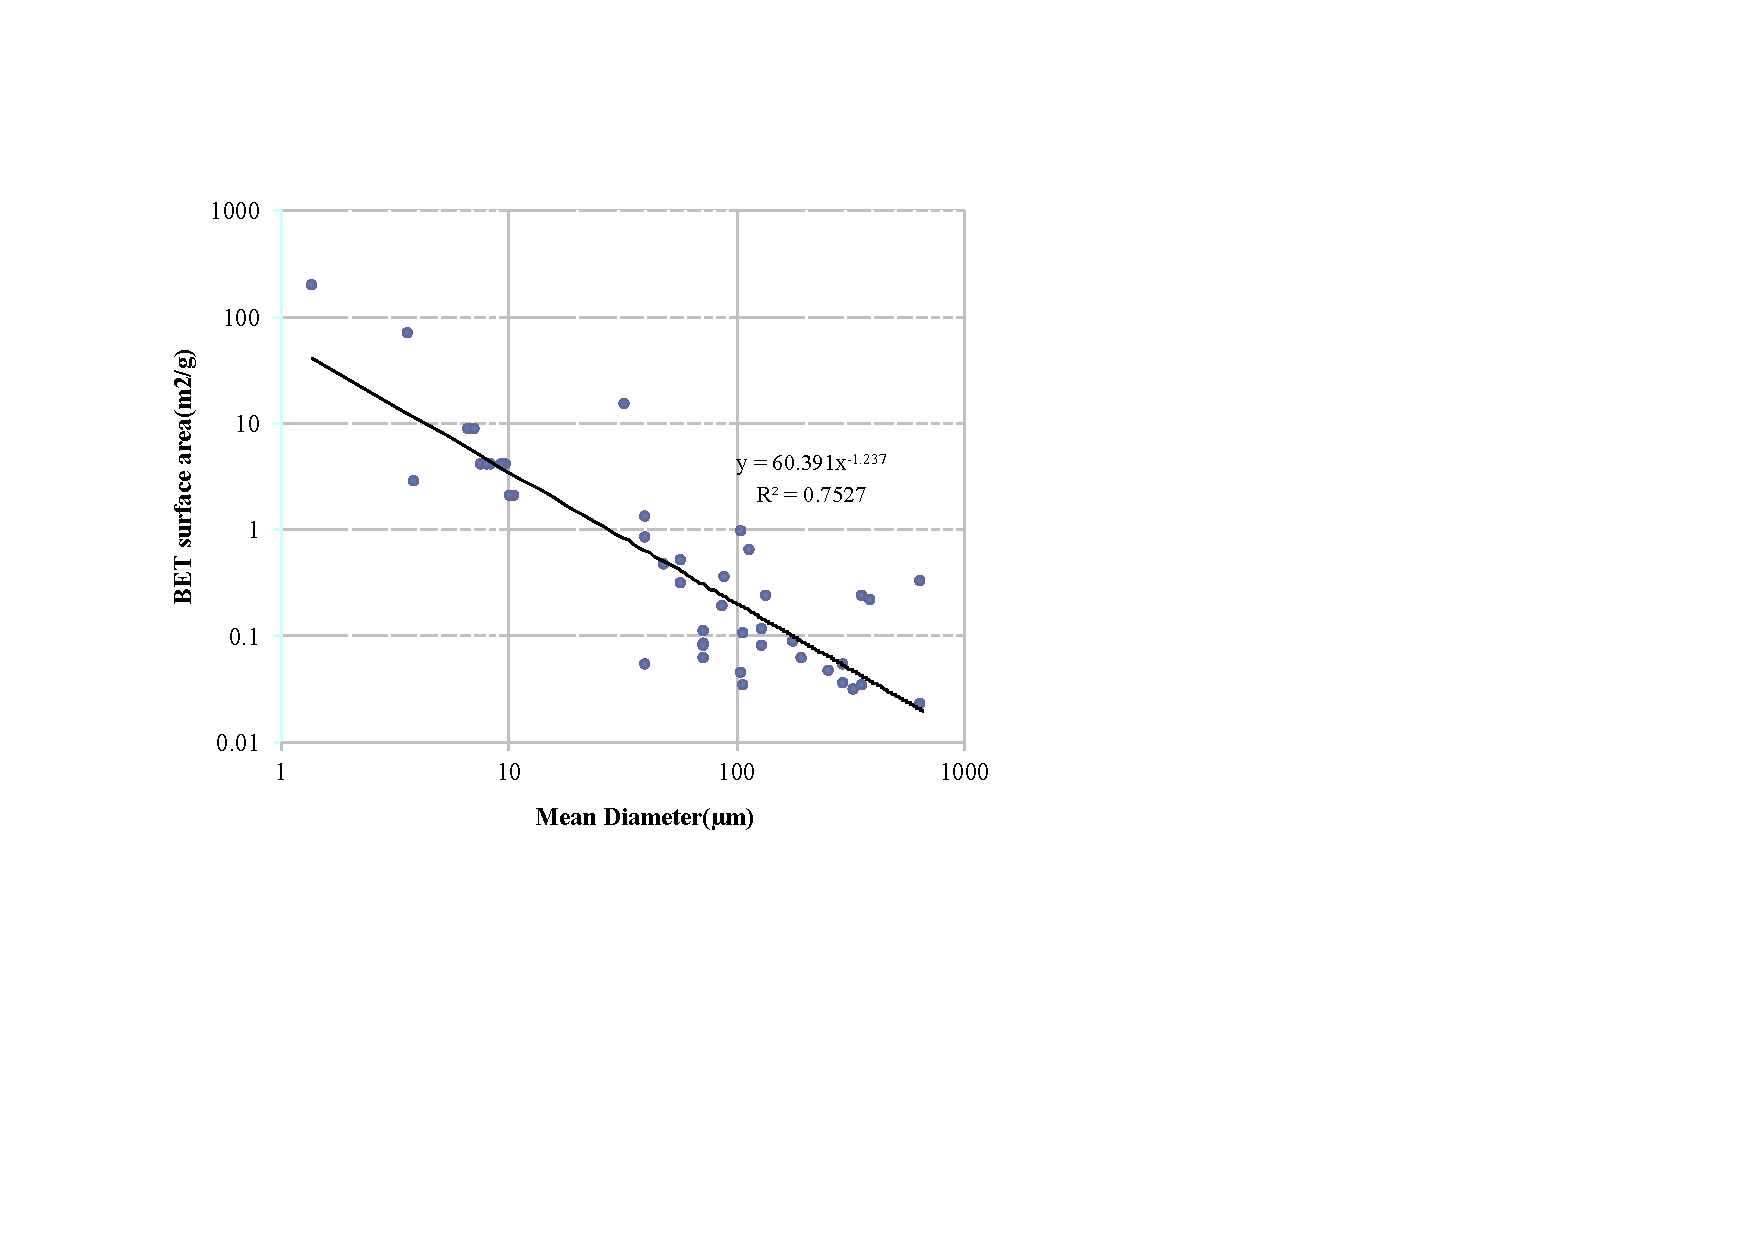
\includegraphics[scale=0.8]{BET_regression.pdf}
\caption{Plot of SSA (\si{\square \metre\per\gram}) measured by BET vs. particle diameter (\si{\micro\meter}) obtained through past studies.}
\label{fig:BET_regression}
\end{figure}

The contribution of each particle fraction to the total of the surface areas is shown in \Cref{fig:app_contri}, for fine grain-type. Particle fractions in the \SIrange[range-units = single,range-phrase = --]{0}{10}{\micro\metre} range contribute \SI{\sim 90}{\percent} of the total of the surface area but only \SI{\sim 33}{\percent} of the total weight. The same particle fraction for coarse contribute \SI{\sim 97}{\percent} and  \SI{\sim 1}{\percent} respectively (not shown here). This highlights the important role of ultrafines in the fine and coarse grain-type.

The total of the surface areas, marked in bold in \Cref{fig:app_contri}, is an estimate of the SSA of the grain-type. The values obtained for the fine and grain-type don't significantly differ from the measured BET values (\Cref{tab:app_concl.}) .

 \begin{table}[h]
   \centering
     \begin{tabular}{ccc}
     \toprule
     \textbf{Grain-type} & \multicolumn{1}{l}{\textbf{Measured SSA (from BET)}} & \multicolumn{1}{l}{\textbf{Estimated SSA}} \\
     \midrule
     Coarse & 1.07 & 2.2 \\
     Fine & 9.78 & 8.89 \\
     \bottomrule
     \end{tabular}%
     
   \caption{Comparison of measured and estimated SSA (\si{\square\metre\per\gram}) }
   \label{tab:app_concl.}%
 \end{table}%

 
\begin{figure}[h]
\centering
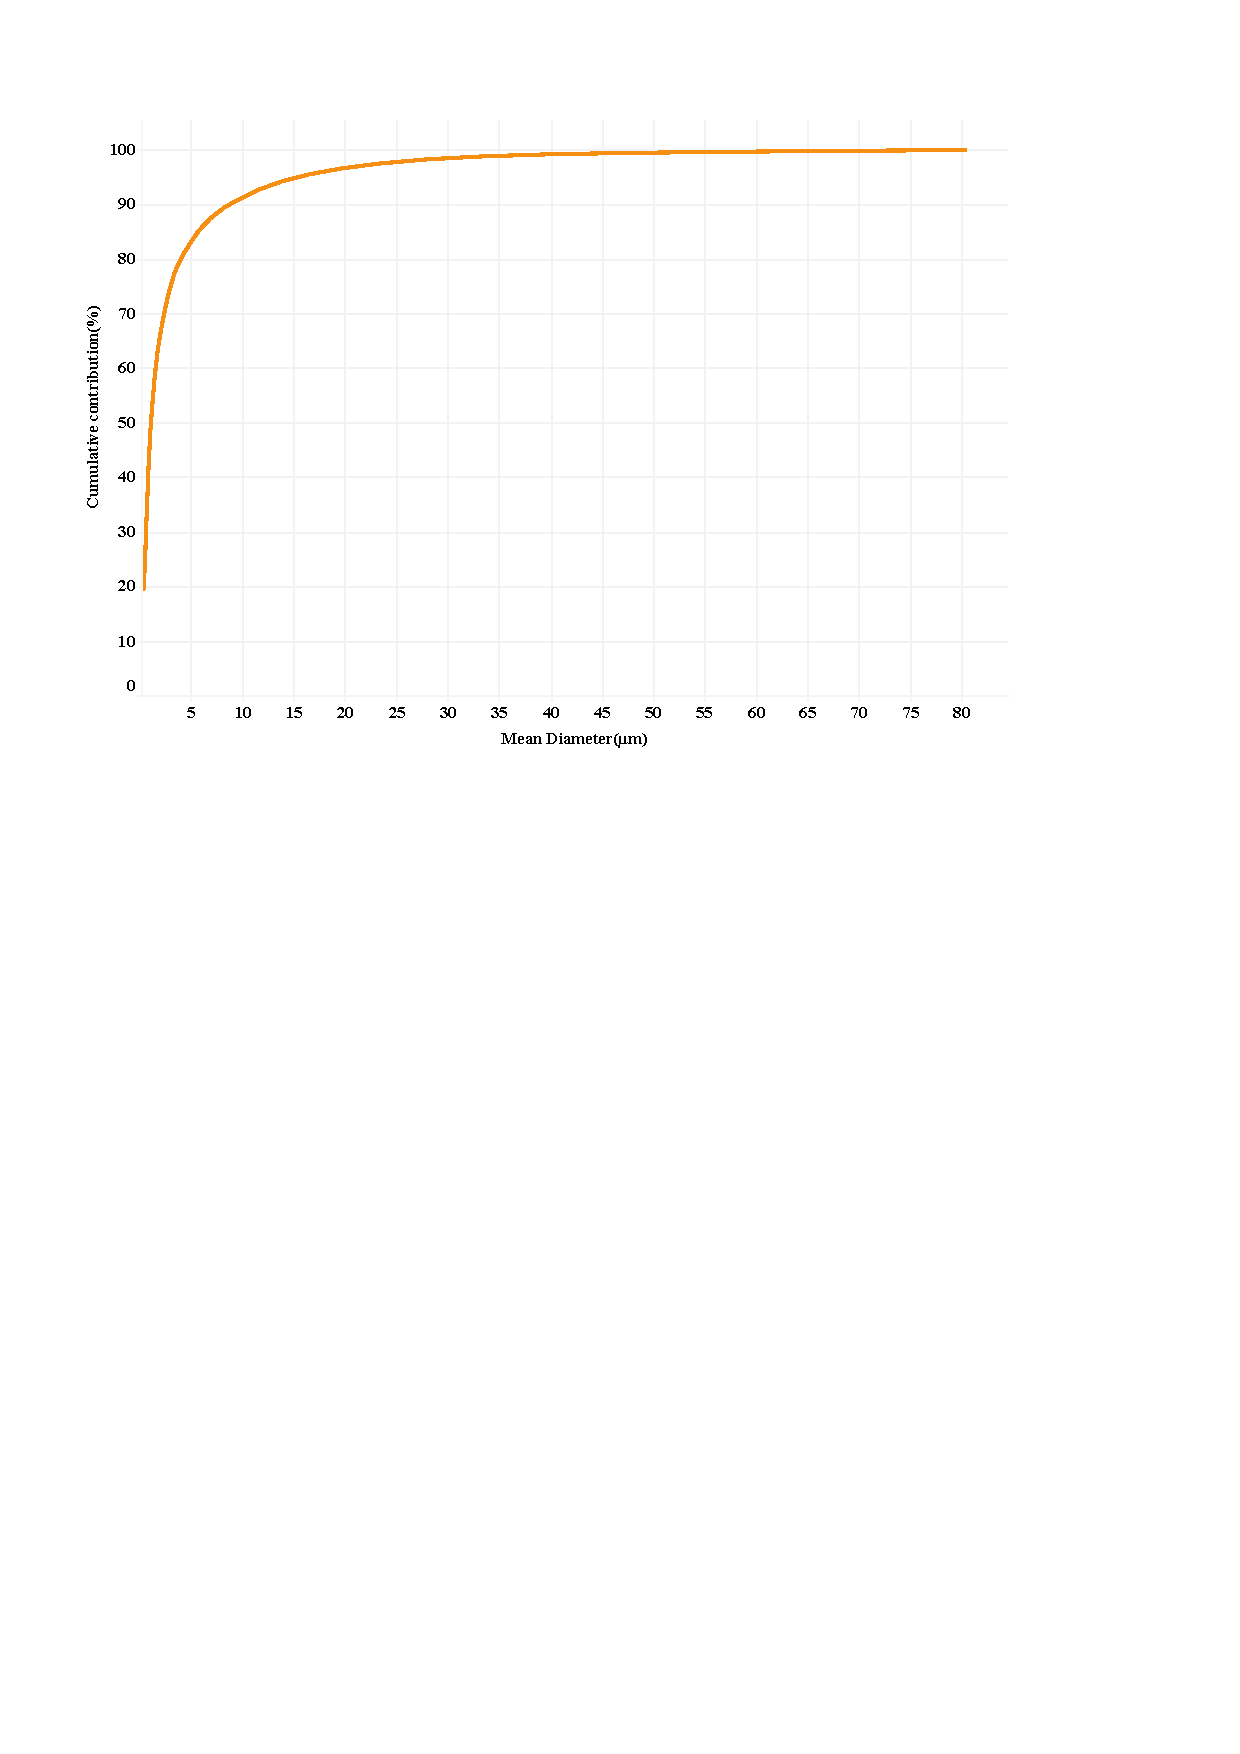
\includegraphics[scale=0.9]{cum_laser_BET_fine.pdf}
\caption{Plot of cumulative contribution of a particle with diameter $D$ to the total of the surface areas (in percent) vs. mean particle diameter (in \si{\micro\meter}) for fine grain-type}
\label{fig:app_contri}
\end{figure}
 
 \begin{table}[h!]
   \centering
     \begin{tabularx}{\linewidth}{|X|X|X|X|}
     \toprule
    \textbf{Mean Diameter (\si{\micro\meter})} & \textbf{Weight fraction} & \textbf{SSA  (from regression equation, \si{\square\meter\per\gram})} & \textbf{Surface area (\si{\square\metre})} \\
    \midrule
     80.30 & 0.053 & 0.266 & 0.014 \\
     67.32 & 0.047 & 0.331 & 0.016 \\
     56.35 & 0.041 & 0.412 & 0.017 \\
     47.39 & 0.043 & 0.511 & 0.022 \\
     39.90 & 0.053 & 0.632 & 0.034 \\
     33.41 & 0.062 & 0.787 & 0.049 \\
     27.93 & 0.067 & 0.982 & 0.066 \\
     23.44 & 0.065 & 1.220 & 0.079 \\
     19.70 & 0.065 & 1.513 & 0.099 \\
     16.45 & 0.063 & 1.890 & 0.119 \\
     13.71 & 0.057 & 2.368 & 0.135 \\
     11.47 & 0.049 & 2.953 & 0.143 \\
     9.73 & 0.038 & 3.619 & 0.138 \\
     8.23 & 0.040 & 4.454 & 0.178 \\
     6.86 & 0.035 & 5.581 & 0.198 \\
     5.74 & 0.030 & 6.960 & 0.211 \\
     4.87 & 0.024 & 8.531 & 0.206 \\
     4.11 & 0.026 & 10.5 & 0.268 \\
     3.36 & 0.027 & 13.5 & 0.359 \\
     2.74 & 0.019 & 17.3 & 0.322 \\
     2.32 & 0.014 & 21.3 & 0.290 \\
     2.00 & 0.012 & 25.7 & 0.313 \\
     1.70 & 0.013 & 31.4 & 0.402 \\
     1.42 & 0.011 & 39.1 & 0.438 \\
     1.20 & 0.009 & 48.3 & 0.445 \\
     1.00 & 0.009 & 60.6 & 0.564 \\
     0.82 & 0.007 & 76.9 & 0.530 \\
     0.70 & 0.004 & 94.1 & 0.423 \\
     0.60 & 0.004 & 113.9 & 0.490 \\
     0.50 & 0.004 & 142.9 & 0.586 \\
     0.34 & 0.008 & 229.1 & 1.742 \\
       &   &   & \textbf{8.894} \\
       \bottomrule
     \end{tabularx}
     \vfill
   
    \caption{Mean diameter and weight fraction from laser granulometry, SSA from regression equation, and surface area as the product of weight fraction and BET area for fine grain-type.}
    \label{tab:app_bet_laser_fine}
 \end{table}

 \begin{table}[h!]
   \centering
     \begin{tabularx}{\linewidth}{|X|X|X|X|}
     \toprule
     \textbf{Mean Diameter (\si{\micro\meter})} & \textbf{Weight fraction} & \textbf{SSA  (from regression equation, \si{\square\meter\per\gram})} & \textbf{Surface area (\si{\square\metre})} \\
     \midrule
     2254.0 & 0.0066 & 0.004 & 0.00003 \\
     1895.5 & 0.0148 & 0.005 & 0.00008 \\
     1595.9 & 0.0325 & 0.007 & 0.00021 \\
     1336.4 & 0.0589 & 0.008 & 0.00048 \\
     1117.0 & 0.0850 & 0.010 & 0.00087 \\
     937.7 & 0.0973 & 0.013 & 0.00124 \\
     787.9 & 0.1072 & 0.016 & 0.00169 \\
     658.2 & 0.1060 & 0.020 & 0.00209 \\
     548.5 & 0.0949 & 0.025 & 0.00234 \\
     458.8 & 0.0774 & 0.031 & 0.00238 \\
     389.2 & 0.0575 & 0.038 & 0.00217 \\
     329.1 & 0.0556 & 0.046 & 0.00258 \\
     274.2 & 0.0439 & 0.058 & 0.00256 \\
     229.4 & 0.0330 & 0.073 & 0.00240 \\
     194.6 & 0.0233 & 0.089 & 0.00207 \\
     164.5 & 0.0214 & 0.110 & 0.00234 \\
     134.4 & 0.0190 & 0.141 & 0.00267 \\
     109.7 & 0.0111 & 0.181 & 0.00201 \\
     92.8 & 0.0069 & 0.222 & 0.00153 \\
     79.8 & 0.0055 & 0.268 & 0.00147 \\
     67.8 & 0.0051 & 0.328 & 0.00167 \\
     56.9 & 0.0043 & 0.408 & 0.00175 \\
     47.9 & 0.0035 & 0.504 & 0.00176 \\
     39.9 & 0.0037 & 0.632 & 0.00234 \\
     32.9 & 0.0031 & 0.802 & 0.00249 \\
     28.0 & 0.0023 & 0.981 & 0.00226 \\
     23.9 & 0.0025 & 1.188 & 0.00297 \\
     19.9 & 0.0026 & 1.491 & 0.00388 \\
     0.5 & 0.0151 & 142.344 & 2.14939 \\
       &   &   & \textbf{2.20} \\
       \bottomrule
     \end{tabularx}
   \caption{Mean diameter and weight fraction from laser granulometry, SSA from regression equation, and surface area as the product of weight fraction and BET area for coarse grain-type.}
   \vfill
   \label{tab:app_bet_laser_coarse}
 \end{table}

\section{Calculation of thickness of the `surface layer'}\label{sec:app_thickness}
The following section calculates the thickness of the Si-rich `surface layer'; using \textbf{coarse} particles as an example. 

Start date of experiment = 5 June 2015\\
Last date of measurement = 14 March 2016\\ 
Number of days water added\footnote{excluding weekends and public holidays}= \SI{274}{days}\\
Water added = \SI{75}{\milli\litre\per\day}\\
Total water added = \num{274} $\times$ \num{75} = \SI{20550}{\milli\litre} = \SI{20.55}{\litre}\\
\ce{Mg^{+2}_{avg,coarse}} (between start and end date) = \SI{590}{\micro\mole\per\litre}\\
Total \ce{Mg^{+2}} released = \num{620} $\times$ \num{20.55} $\times$ \num{e-6}\si{\mole} = \SI{0.0127}{\mole}\\				
Molecular Mass of Mg = \SI{24.3}{\gram\per\mole}\\
\textbf{Total \ce{Mg^{+2}} released = \num{0.0127} $\times$ \num{24.3}  =  \SI{0.31}{\gram}}\\

\noindent At stochiometry, Total $\mathrm{Si_{released}}$ = $\textfrac{0.0127}{1.88}$= \SI{0.00676}{\mole}\\
Molecular mass of dissolved silica (\ce{H_4SiO_4}) = \SI{96.11}{\gram\per\mole}\\
Total $\mathrm{Si_{released}}$ = \num{0.00676}$\times$ \num{96.11}= \SI{0.65}{\gram} \\
Observed $\mathrm{Si_{avg}}$ = \SI{9.8}{\micro\mole\per\litre}\\
Total \;$\mathrm{Si_{observed}}$ = 9.8 $\times$ 20.55 = \SI{201.39e-6}{\mole}\\
Total$\mathrm{Si_{observed}}$ = 201.39 $\times$ 96.11 $\times$ \SI{e-6}{\gram} = \SI{0.019}{\gram}\\
Total $\mathrm{Si_{precipitated}}$ = Total $\mathrm{Si_{released}}$ - Total$\mathrm{Si_{observed}}$\\ 
$\mathrm{Si_{precipitated}}$ = 0.65 \ - \ 0.019 = \SI{0.631}{g}

\noindent Assuming that all $\mathrm{Si_{precipitated}}$ forms a uniform layer of Si around the mineral surface:\\
Density of Si-layer = \SI{1.32}{\gram\per\cubic\centi\meter}\\
Average TSA of coarse particles = \SI{1041.95}{m^2}\\
$\mathrm{Mass_{Si} = Density_{Si} \times Volume_{Si}}$ \\
$\mathrm{Volume_{Si} = Thickness_{Si} \times TSA}$\\[0.3cm]
$\mathrm{Thickness_{Si}=\frac{Mass_{Si}}{Density_{Si}\times TSA}}$\\[0.3cm]
$\mathrm{Thickness_{Si}}$ = $\textfrac{0.631}{1.32$\times$ 1041.95}$ $\times$ \num{e-4} \si{cm} = \SI{4.7e-8}{cm} = \SI{4.7e-10}{m}  = \SI{0.47}{nm}\\[0.3cm]
A similar calculation can be done for fine and mixed particles.

\begin{table}[htbp]
  \centering
  
    \begin{tabular}{ccccccc}
    \toprule
      & \textbf{\ce{Mg_{obs}} (g)} & \textbf{\ce{Si_{released}}(g)} & \textbf{\ce{Si_{observed}}(g)} & \textbf{\ce{Si_{ppt}}(g)} & \textbf{Avg. TSA (\si{\square\meter})} & \textbf{Thickness} (\si{\nano\meter}) \\
      \midrule
    \textbf{coarse} & 0.31 & 0.65 & 0.019 & 0.63 & 1041.95 & 0.47 \\
    \textbf{fine } & 0.75 & 1.58 & 0.018 & 1.56 & 6246.6 & 0.19 \\
    \textbf{mixed} & 0.65 & 1.37 & 0.024 & 1.35 & 4771.5 & 0.21 \\
    \bottomrule
    \end{tabular}
  \label{tab:results_thickness}
  \caption{Results for Mg and Si released, observed, and precipitated. The Si precipitated converted to thickness of layer.}
\end{table}

\section{Minor ion analysis}\label{sec:app_minor_ion}

The concentration profiles with time (Date), for the minor cations - \ce{Ca^{+2}}, \ce{K+}, and \ce{Na+} and minor anions -  \ce{NO3^{-}}, \ce{Cl-}, and \ce{SO4^{2-}} are plotted in \Cref{fig:app_cations,fig:app_anions} respecitvely.

\begin{figure}[h]
\centering
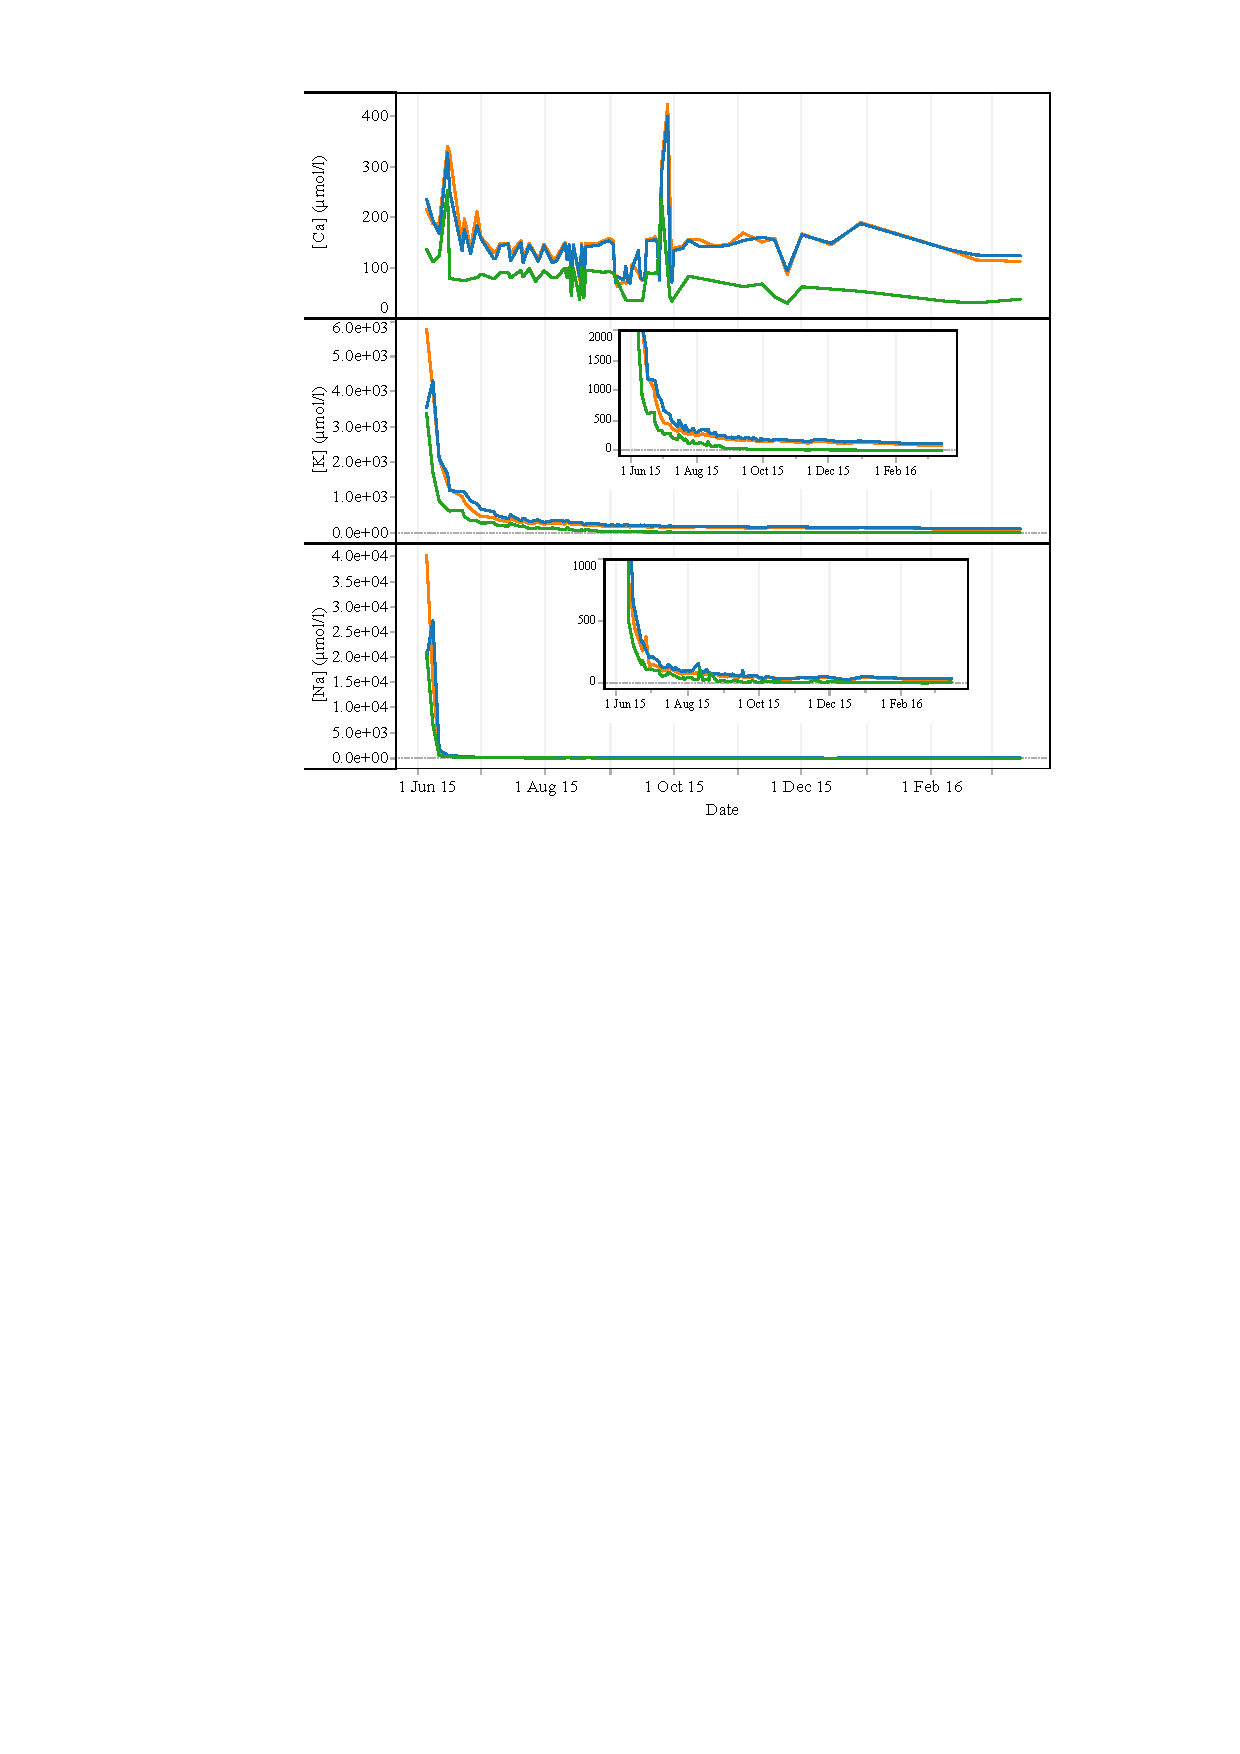
\includegraphics[scale=1.3]{cations.pdf}
\caption{The concentration of minor ions - \ce{Ca^{+2}}, \ce{K+}, and \ce{Na+} with time (Date), averaged over the three grain types - fine, coarse, and mixed.}
\label{fig:app_cations}
\end{figure}

\begin{figure}[h]
\centering
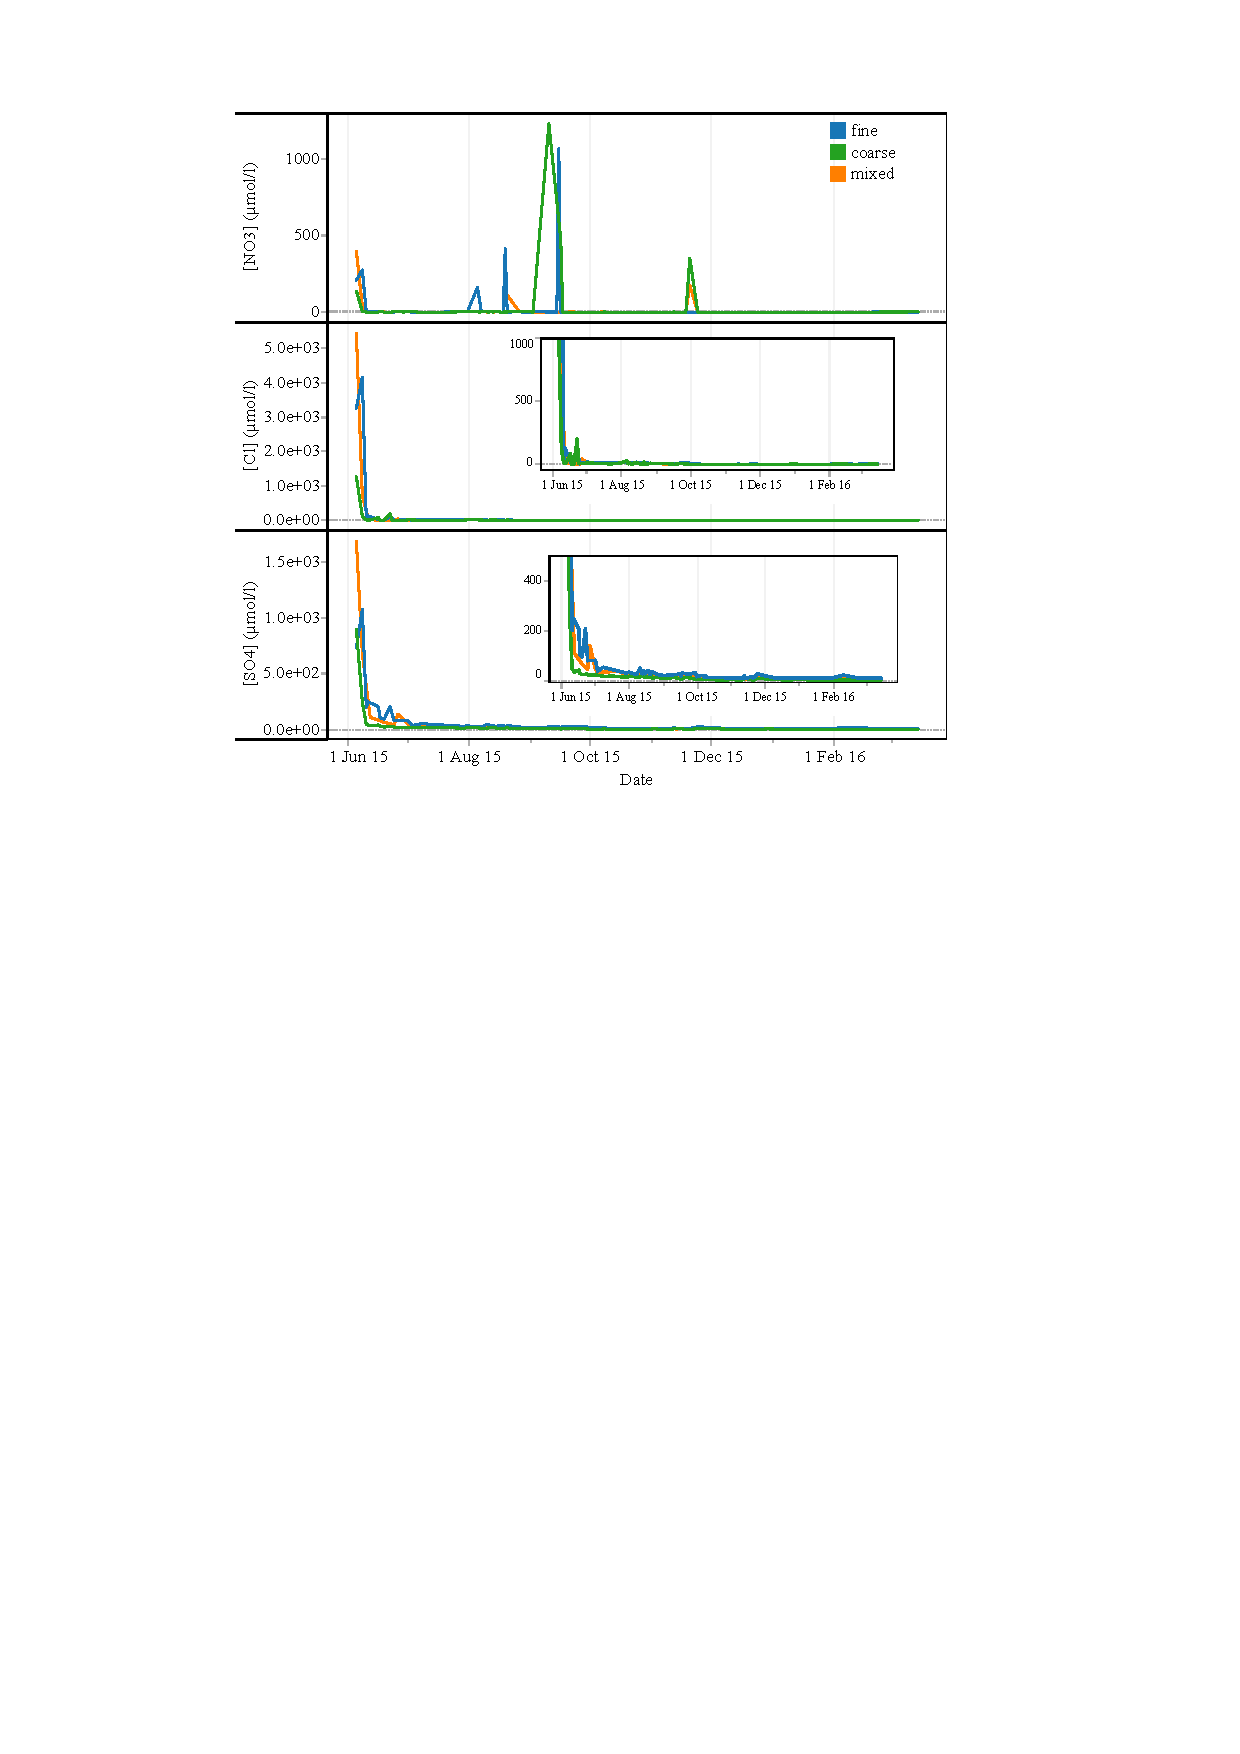
\includegraphics[scale=1.3]{anions.pdf}
\caption{The concentration of minor ions - \ce{NO3^{-}}, \ce{Cl-}, and \ce{SO4^{2-}} with time (Date), averaged over the three grain types - fine, coarse, and mixed.}
\label{fig:app_anions}
\end{figure}

 
